\documentclass{article}
\usepackage{graphicx}
\usepackage{float}
\usepackage{geometry}
\usepackage{tcolorbox}
\usepackage{amssymb} 
\usepackage{wasysym}
\usepackage{subcaption}
\usepackage{bm}
\usepackage{booktabs} 
\definecolor{lightgray}{gray}{0.9} % Define lightgray color
\geometry{left=0.8in,right=0.8in,top=0.8in,bottom=1in}

\title{Experiment 1: Experimentation \& Evaluation 2023}
\author{Your Name}
\date{\today}

\begin{document}
\maketitle

Short (120-130 words) summary of your entire report. Give the reader a quick idea of what you did and what the main findings were (if you prepare this report ahead of time, leave out the findings until after you finish the analysis).


\section{Introduction}
Bubble Inc., a software development company specializing in Java utilities, is faced with the crucial decision of selecting a sorting algorithm for inclusion in their upcoming library. The company has identified three candidate algorithms: BubbleSortPassPerItem, BubbleSortUntilNoChange, and BubbleSortWhileNeeded, all implementing the Sorter interface. The primary criterion for the selection process is performance, specifically the execution time required by each algorithm, with lower execution times being preferable.\\
To address this decision, we have designed a comprehensive experiment aimed at rigorously assessing the performance of the three sorting algorithms. While the choice of sorting algorithm is the primary independent variable, we also consider the manipulation of additional independent variables, such as the type of data in the array to be sorted and the array behaviour (random, sorted, partSorted, reverse, duplicates, noDuplicates, equal).\\
The experiment involves multiple repetitions of measurements to ensure statistical reliability. In this report, we present a detailed account of the experimental design, methodology, and the results obtained through careful analysis.\\
This experiment aims not only to contribute valuable insights to Bubble Inc.'s decision-making process but also to adhere to best practices in experimental design, ensuring transparency, reproducibility, and reliability in the assessment of sorting algorithm performance.


\begin{tcolorbox}[title=Hypotheses:, colback=white, colframe=black, arc=0pt, outer arc=0pt]
    Write down your (falsifiable!) hypotheses here. Each hypothesis must include independent and your dependent variables. You must write down your hypotheses before you do your experiment!
\end{tcolorbox}

\section{Method}
In the following subsections, describe everything that a reader would need to replicate your experiment in all important details.
\subsection{Variables}
Explicitly identify the independent variable(s) (i.e., what you as the experimenter manipulate): 

    \begin{tcolorbox}[title=Independent Variable:, colback=white, colframe=black, arc=0pt, outer arc=0pt]
        \begin{itemize}
         \item[1.] \textbf{Sorting Algorithm (Algorithm Type):}
            \begin{itemize}
            \item BubbleSortPassPerItem
            \item BubbleSortUntilNoChange
            \item BubbleSortWhileNeeded
            \end{itemize}
        \item[2.] \textbf{Data Type (Type):}
            \begin{itemize}
            \item int
            \item Integer
            \item String
            \item double
            \item char
            \item byte
            \end{itemize}
        \item[3.] \textbf{Array Characteristics (Type of the Array):}
            \begin{itemize}
            \item random
            \item sorted
            \item partially sorted
            \item reverse sorted
            \item with duplicates
            \item with no duplicates
            \item with equal elements
            \end{itemize}
        \end{itemize}

    \end{tcolorbox}
Explicitly identify the dependent variable(s) (i.e., what you measure):\\

\begin{tcolorbox}[title=Dependent Variable:, colback=white, colframe=black, arc=0pt, outer arc=0pt]
    \begin{itemize}
        \item[1.] \textbf{Execution Time:}
        \begin{itemize}
            \item Measured in nanoseconds, capturing the time taken by each sorting algorithm to complete the sorting process.
        \end{itemize}
    \end{itemize}
\end{tcolorbox}

\subsection{Design}
Check off the characteristics of your experimental design:\\

\textbf{Type of Study} (check one):\\
\noindent
\begin{minipage}{0.4\textwidth}
    \fbox{\Square{} \textbf{Observational Study}}
\end{minipage}%
\begin{minipage}{0.4\textwidth}
    \fbox{\Square{} \textbf{Quasi-Experiment}}
\end{minipage}%
\begin{minipage}{0.2\textwidth}
    \fbox{\bm{\XBox{}} \textbf{Experiment}}
\end{minipage}\\\\
Conducted controlled experiments with intentional manipulation of variables to assess the performance of sorting algorithms.

In within-subjects (or 'repeated measures') designs, each participant is exposed to all of the conditions of the experiment.

In our experiment, we test each algorithm (\texttt{BubbleSortPassPerItem}, \texttt{BubbleSortUntilNoChange}, \texttt{BubbleSortWhileNeeded}) for each combination of the element type of the array with different characteristics of the array.

This means that each algorithm is tested for:

\begin{itemize}
    \item (\texttt{int}, [random, sorted, partially sorted, reverse sorted, with duplicates, with no duplicates, equal elements]),
    \item (\texttt{Integer}, [random, sorted, partially sorted, reverse sorted, with duplicates, with no duplicates, equal elements]),
    \item (\texttt{String}, [random, sorted, partially sorted, reverse sorted, with duplicates, with no duplicates, equal elements]),
    \item (\texttt{double}, [random, sorted, partially sorted, reverse sorted, with duplicates, with no duplicates, equal elements]),
    \item (\texttt{char}, [random, sorted, partially sorted, reverse sorted, with duplicates, with no duplicates, equal elements]),
    \item (\texttt{byte}, [random, sorted, partially sorted, reverse sorted, with duplicates, with no duplicates, equal elements]).
\end{itemize}

Furthermore, it has repeated measures because each of the previous array-type combinations is tested 150 times, for which the first 25 iterations are not counted as actual values but as warm-up values.
\\\\
\textbf{Number of Factors} (check one):\\
\noindent
\begin{minipage}{0.4\textwidth}
    \fbox{\Square\ \textbf{Single-Factor Design}}
\end{minipage}%
\begin{minipage}{0.4\textwidth}
    \fbox{\bm{\XBox{}} \textbf{Multi-Factor Design}}
\end{minipage}%
\begin{minipage}{0.0\textwidth}
    \fbox{\Square\ \textbf{Other}}
\end{minipage}\\\\
- Investigated the impact of multiple independent variables, including the sorting algorithm, data type, and array characteristics.
\begin{figure}[H]
    \centering
    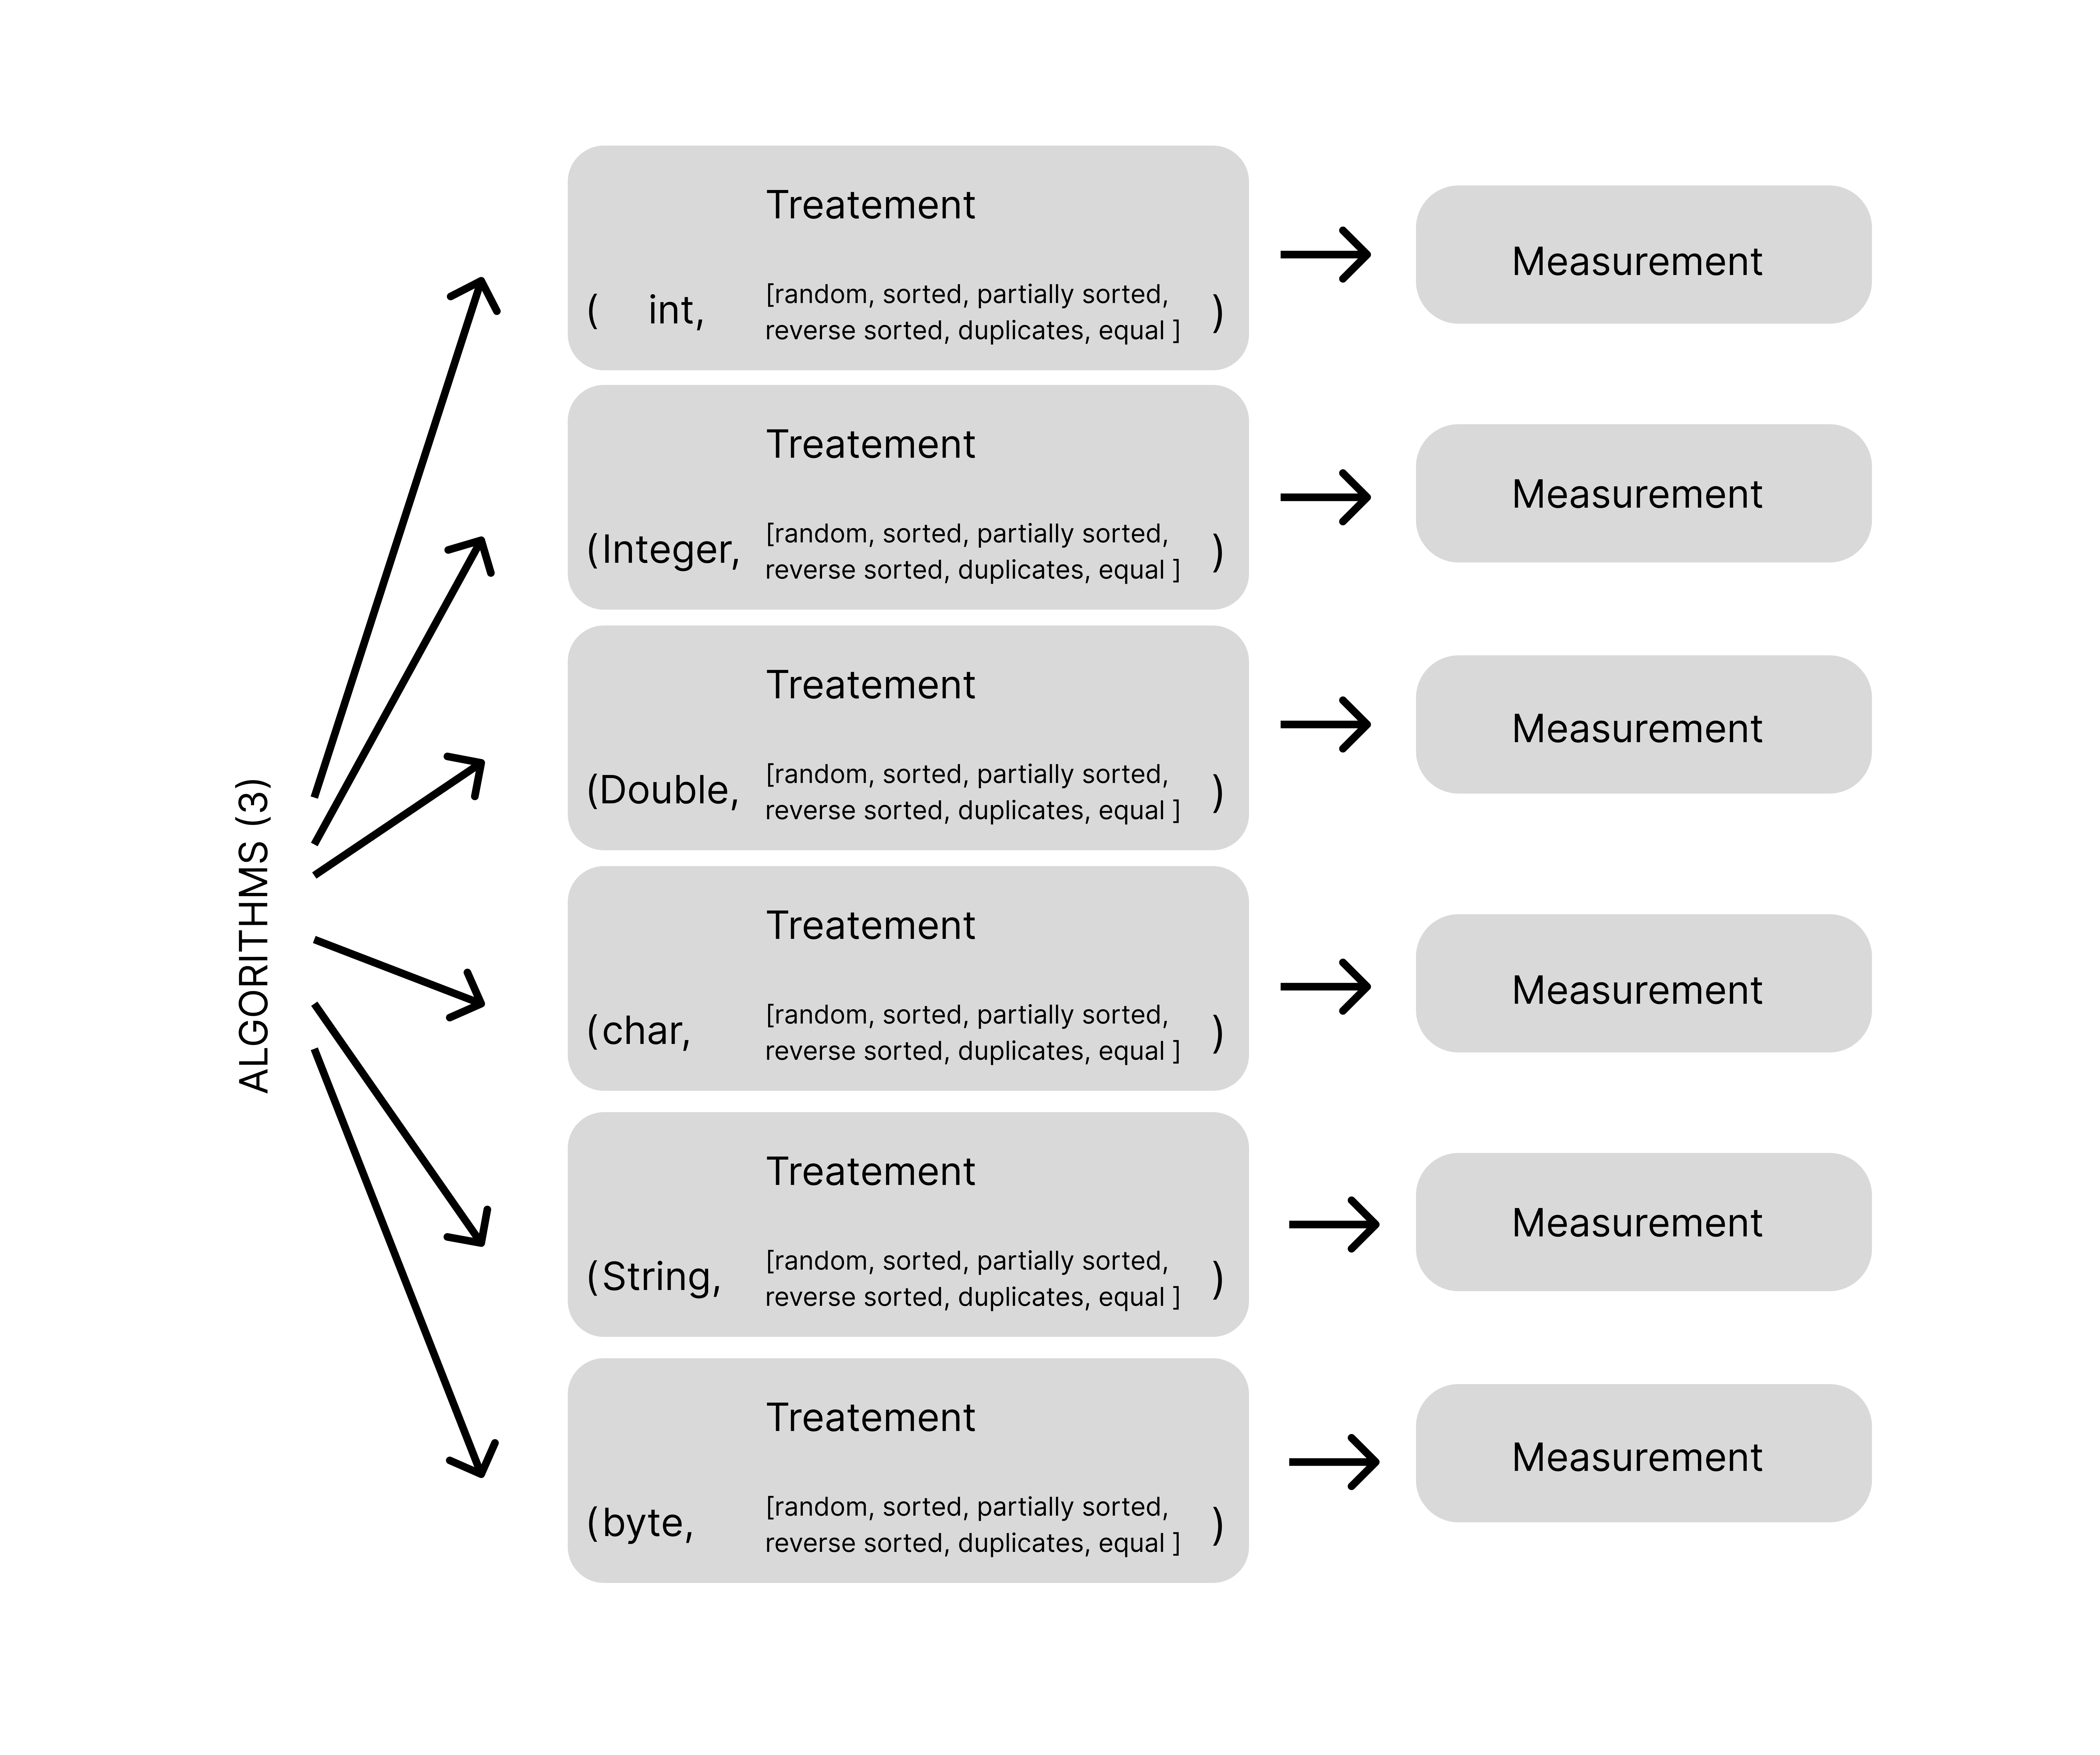
\includegraphics[width=\textwidth]{./data/Group12.png}
    \caption{Multi-factor design}
\end{figure}

\subsection{Apparatus and Materials}
Describe in sufficient detail any relevant “props” that you used in your experiment. This could be the computer you used (exact model and specification), the software used (URL, version numbers), the way you measured, e.g., time (A stopwatch? A background process on the computer that got automatically triggered?). Omit needless detail (e.g., think whether details like the size of the table the laptop was placed on, or the hard disk size, might have affected your results or not).
\begin{itemize}
  \item \textbf{Sorting Algorithms:}
    \begin{itemize}
      \item Utilized three sorting algorithms:
        \begin{itemize}
          \item BubbleSortPassPerItem
          \item BubbleSortUntilNoChange
          \item BubbleSortWhileNeeded
        \end{itemize}
    \end{itemize}
     All algorithms implement the Sorter interface.

  \item \textbf{Data Types:}
    \begin{itemize}
      \item Evaluated various data types, including:
        \begin{itemize}
          \item int
          \item Integer
          \item String
          \item double
          \item char
          \item Byte
        \end{itemize}
    \end{itemize}

  \item \textbf{Array Characteristics:}
    \begin{itemize}
      \item Generated arrays with different characteristics:
        \begin{itemize}
          \item random
          \item sorted
          \item partSorted
          \item reverse
          \item duplicates
          \item noDuplicates
          \item equal
        \end{itemize}
    \end{itemize}

  \item \textbf{Measurement Tool:}
    \begin{itemize}
      \item Employed \texttt{System.nanoTime()} for precise measurement of execution time.
      \item Employed \texttt{System.currentTimeMillis()} for program measurements time. 
      \item Employed a stopwatch to measure again the time the program took.
    \end{itemize}
    
    \item \textbf{Machine used:}
    \begin{itemize}
      \item Hardware Model: \texttt{Dell Inc. Precision 5550}
      \item Firmware version: \texttt{1.24.1}
      \item Processor: \texttt{Intel® Core™ i7-10850H × 12}
      \item OS name: \texttt{Ubuntu 23.04}
      \item OS type: \texttt{64-bit}
      \item Kernel version: \texttt{Linux 6.2.0-36-generic}
    \end{itemize}
\end{itemize}



\subsection{Procedure}
Describe how you used your props and/or the participants to perform your actual experiment, i.e., how you actually carried out a single experimental run. What was done to the participants? What did they have to do? How long did each session take (unless this is an actual dependent variable)? If you did not have participants, explain, e.g., what software was started by whom in what order.
\begin{itemize}
  \item[1.] \textbf{Algorithm Implementation:}
    \begin{itemize}
      \item Implemented BubbleSortPassPerItem, BubbleSortUntilNoChange, and BubbleSortWhileNeeded algorithms.
    \end{itemize}

  \item[2.] \textbf{Array Generation:}
    \begin{itemize}
      \item Created arrays of varying types and characteristics using the \texttt{arrayGeneratorGeneral} method.
    \end{itemize}

  \item[3.] \textbf{Sorting Performance Analysis:}
    \begin{itemize}
      \item Repeated sorting processes 150 times for each combination of algorithm, data type, and array characteristics.
      \item Executed the sorting algorithms on generated arrays and recorded the execution time.
    \end{itemize}

  \item[4.] \textbf{Data Collection:}
    \begin{itemize}
      \item Collected and stored execution time data for analysis and reporting.
      \item Limited data recording to after the 25th iteration to ensure stabilized results.
    \end{itemize}

  \item[5.] \textbf{CSV Result Logging:}
    \begin{itemize}
      \item Logged the experiment results, including algorithm type, data type, array order, start time, end time, and elapsed time, into a CSV file (\texttt{results1000.csv/results10000.csv}).
    \end{itemize}
\end{itemize}
Times taken for the experiment:
    \begin{itemize}
     \item For array dimension of 1000: 20 minutes ($10:10 \rightarrow 10:30$)
     \item For array dimension of 10000: 2 hours ($10:37 \rightarrow 12:35$)
    \end{itemize}

\section{Results}
\subsection{Visual Overview}

Below, we present graphs representing the distribution of our data obtained through testing three different algorithms with various independent variables. The graphs are categorized into two groups: the first group represents data collected with an array dimension of 1000, while the second group represents data collected with an array dimension of 10000.\\

We have chosen to display the graphs using Boxen plots due to their ability to offer a detailed representation of the dataset's distribution. This choice is particularly advantageous for large datasets as Boxen plots provide enhanced visibility into distribution tails and varying data densities.\\
\begin{figure}[H]
    \centering
    \begin{subfigure}[b]{0.48\textwidth}
        \centering
        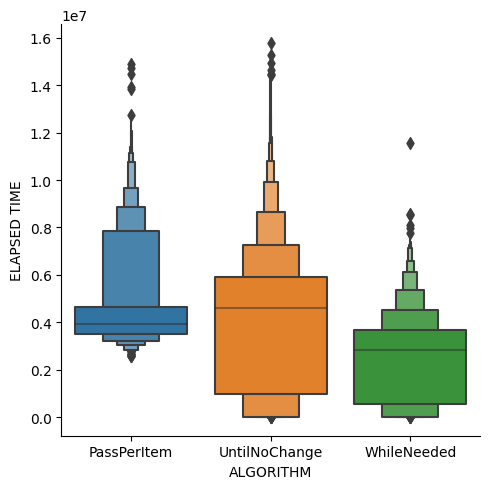
\includegraphics[width=\textwidth]{./data/comparison_algorithm_1000.png}
        \caption{Array dimension = 1000}
    \end{subfigure}
    \hfill
    \begin{subfigure}[b]{0.48\textwidth}
        \centering
        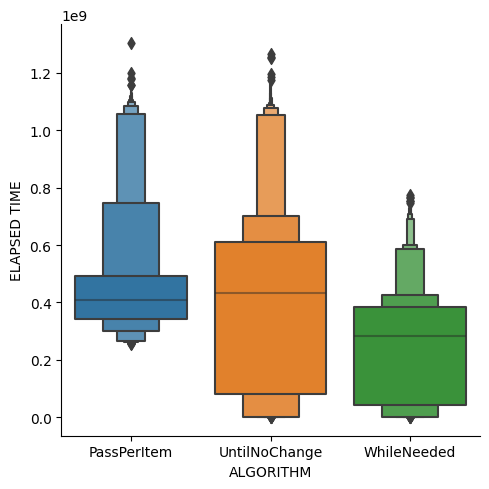
\includegraphics[width=\textwidth]{./data/comparison_algorithm_10000.png}
        \caption{Array dimension = 10000}
    \end{subfigure}
    \caption{Graphs Algorithms Comparison}
\end{figure}

Here, we present graphs representing the distribution of our data obtained by testing three different algorithms. In both dimensions, the dense part of the data covers almost the same range, albeit on different scales. The array with a dimension of 1000 elements is on the scale of seconds multiplied by $10^{-2}$, while the array with a dimension of 10000 elements is on the scale of seconds.\\

From these two graphs, we can infer that, generally, regardless of the array type or dimension, the WhileNeededAlgorithm consistently emerges as the fastest.\\

Next, we explore how the algorithms perform with different types of arrays and different array orders.\\
\begin{figure}[H]
    \centering
    \begin{subfigure}[b]{0.48\textwidth}
        \centering
        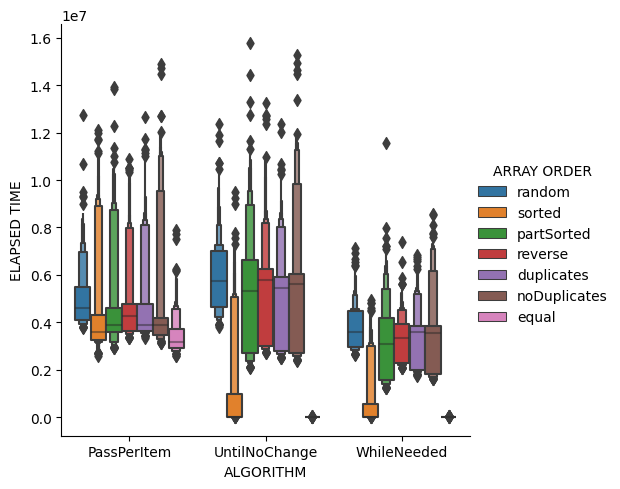
\includegraphics[width=\textwidth]{./data/array_order_1000.png}
        \caption{Array dimension = 1000}
    \end{subfigure}
    \hfill
    \begin{subfigure}[b]{0.48\textwidth}
        \centering
        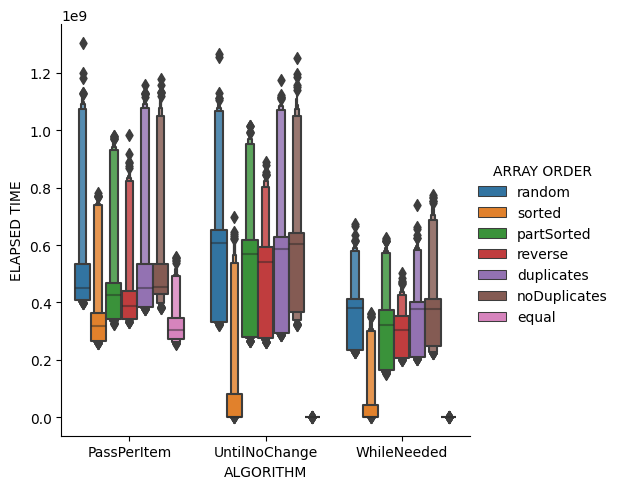
\includegraphics[width=\textwidth]{./data/array_order_10000.png}
        \caption{Array dimension = 10000}
    \end{subfigure}
    \caption{Graph Array order Comparison between algorithms} 
\end{figure}

From these two graphs, we can observe the distinct sorting approaches employed by the three algorithms. For instance, when focusing on the array order "sorted," it becomes evident that the UntilNoChange and WhileNeeded algorithms outperform the PassPerItem algorithm. This suggests that, in many instances and depending on the array type, the former two algorithms efficiently traverse the array and return results swiftly. In contrast, the PassPerItem algorithm, with its need to compare each element and undergo a specified number of passes, experiences reduced efficiency.\\

Shifting our focus to the remaining array orders, we notice that they all closely align with the dense part of the first graph, which provides a general comparison of the three algorithms.\\

In the last two graphs, we illustrate the differences between various array types. Notably, the WhileNeededAlgorithm and UntilNoChange algorithms exhibit a broad distribution along the y-axis (elapsed time), likely influenced by the varying array orders. On the other hand, irrespective of array type and order, the other algorithm's data is more concentrated within a specific range.\\
\begin{figure}[H]
    \centering
    \begin{subfigure}[b]{0.48\textwidth}
        \centering
        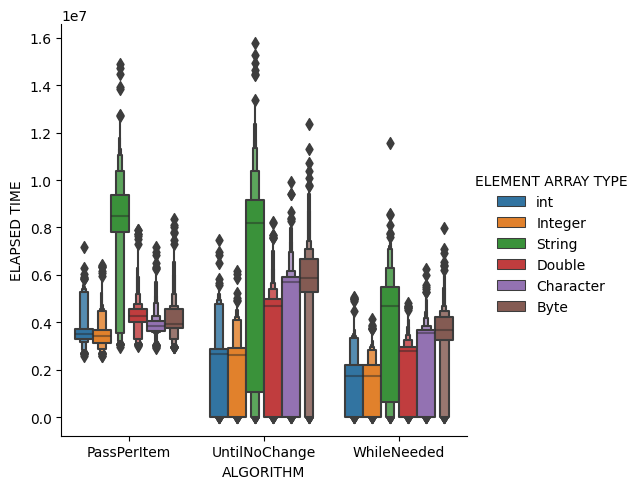
\includegraphics[width=\textwidth]{./data/array_type_1000.png}
        \caption{Array dimension = 1000}
    \end{subfigure}
    \hfill
    \begin{subfigure}[b]{0.48\textwidth}
        \centering
        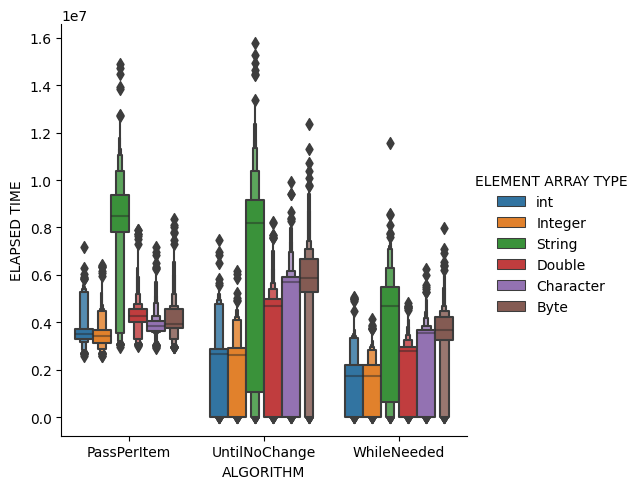
\includegraphics[width=\textwidth]{./data/array_type_10000.png}
        \caption{Array dimension = 1000}
    \end{subfigure}
    \caption{Graph Array type Comparison between algorithms}
\end{figure}
\subsubsection{Standard Deviantion Calculation}

Below, you'll find the standard deviation calculations for the mean of the elapsed time among algorithms.\\

We opted to use standard deviation instead of absolute deviation because standard deviation is more sensitive to values that deviate significantly from the mean compared to absolute deviation.\\

The standard deviation is calculated using the following formula:
\[ \sigma = \sqrt{\frac{\sum_{i=1}^{n}(x_i - \bar{x})^2}{n-1}} \]

Below, we observe the differences in the standard deviation of the mean elapsed time among algorithms for array dimensions of both 1000 and 10000.\\


\begin{figure}[H]
    \centering
    \begin{subfigure}[b]{0.48\textwidth}
        \centering
        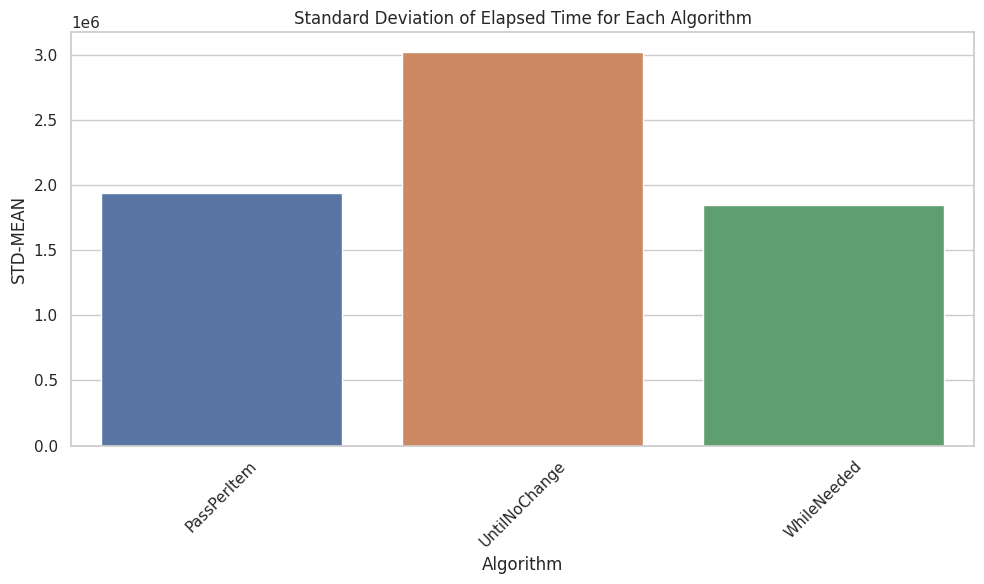
\includegraphics[width=\textwidth]{./data/std_algo_1000.png}
        \caption{Array dimension = 1000}
    \end{subfigure}
    \hfill
    \begin{subfigure}[b]{0.48\textwidth}
        \centering
        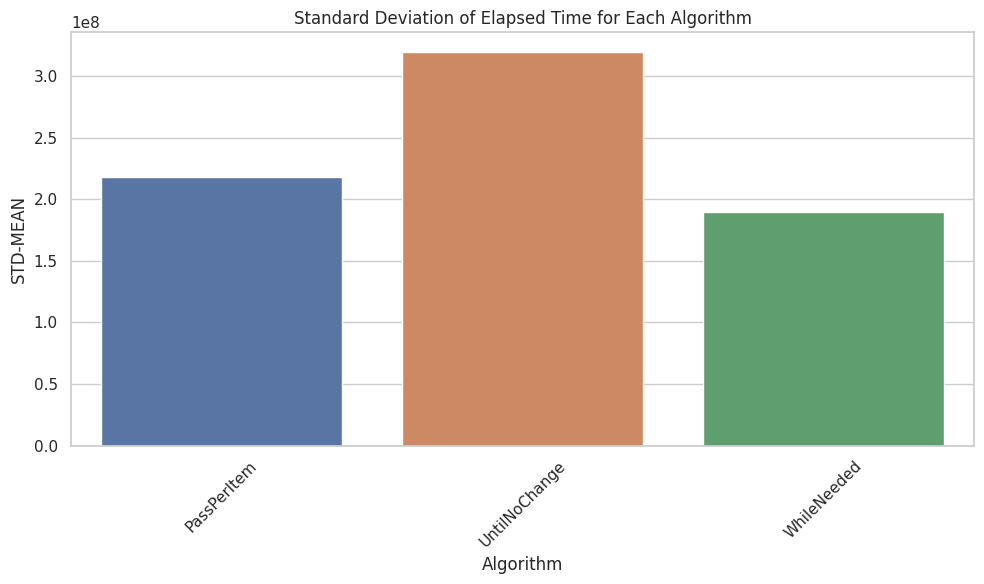
\includegraphics[width=\textwidth]{./data/std_algo_10000.png}
        \caption{Array dimension = 10000}
    \end{subfigure}
    \caption{STD Mean of elapsed time between algorithms}
\end{figure}

Across both dimensions, the WhileNeededAlgorithm consistently demonstrates its efficiency, confirming it as the most efficient algorithm on average.

\begin{table}[h]
  \centering
  \caption{Standard Deviation of Elapsed Time for Each Algorithm}
  \begin{tabular}{lccc}
    \toprule
    Algorithm & STD-MEAN (10,000) & STD-MEAN (1,000) \\
    \midrule
    PassPerItem & $2.177038 \times 10^8$ & $1.940991 \times 10^6$ \\
    UntilNoChange & $3.194608 \times 10^8$ & $3.019103 \times 10^6$ \\
    WhileNeeded & $1.892941 \times 10^8$ & $1.847857 \times 10^6$ \\
    \bottomrule
  \end{tabular}
\end{table}
Here, we present the standard deviation of the elapsed time for each algorithm with various types of arrays and different array orders:\\
\begin{figure}[H]
  \centering
  \begin{subfigure}[b]{0.48\textwidth}
      \centering
      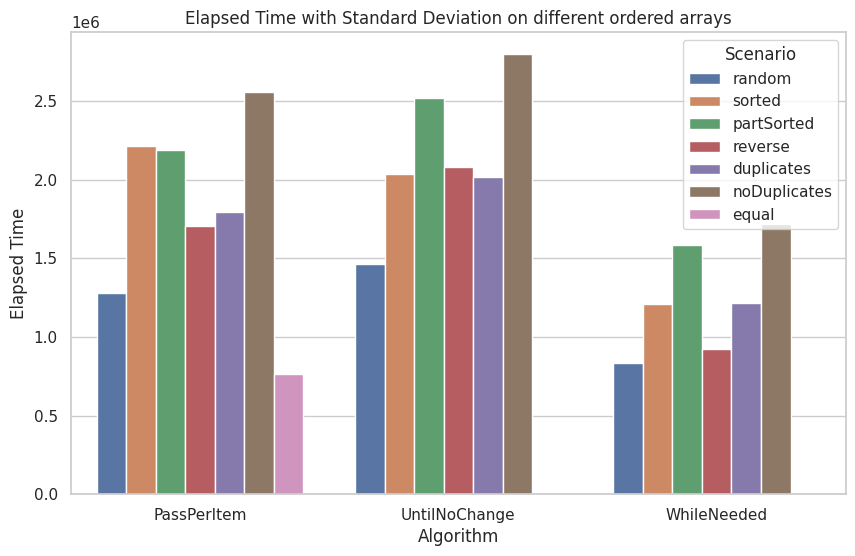
\includegraphics[width=\textwidth]{./data/std_order_array_1000.png}
      \caption{Array dimension = 1000}
  \end{subfigure}
  \hfill
  \begin{subfigure}[b]{0.48\textwidth}
      \centering
      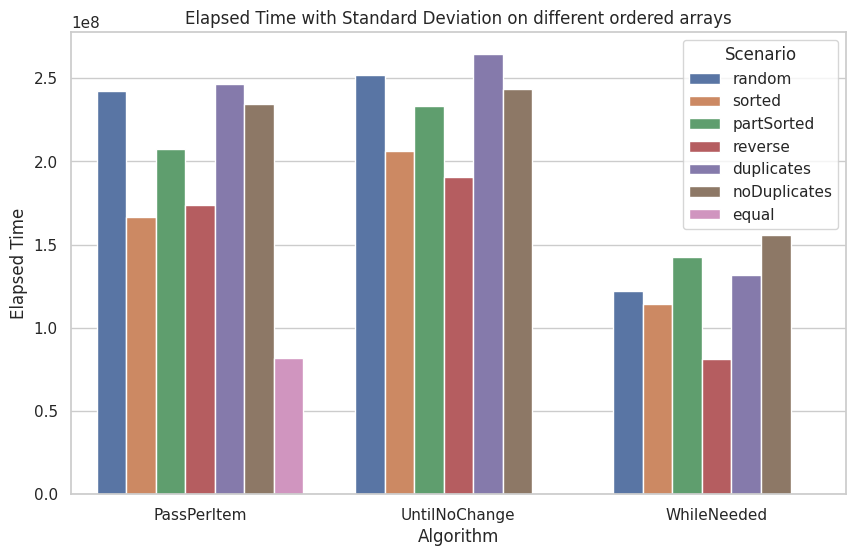
\includegraphics[width=\textwidth]{./data/std_order_array_10000.png}
      \caption{Array dimension = 10000}
  \end{subfigure}
  \caption{STD Mean of elapsed time of Array Order between algorithms}
\end{figure}


\begin{figure}[H]
    \centering
    \begin{subfigure}[b]{0.48\textwidth}
        \centering
        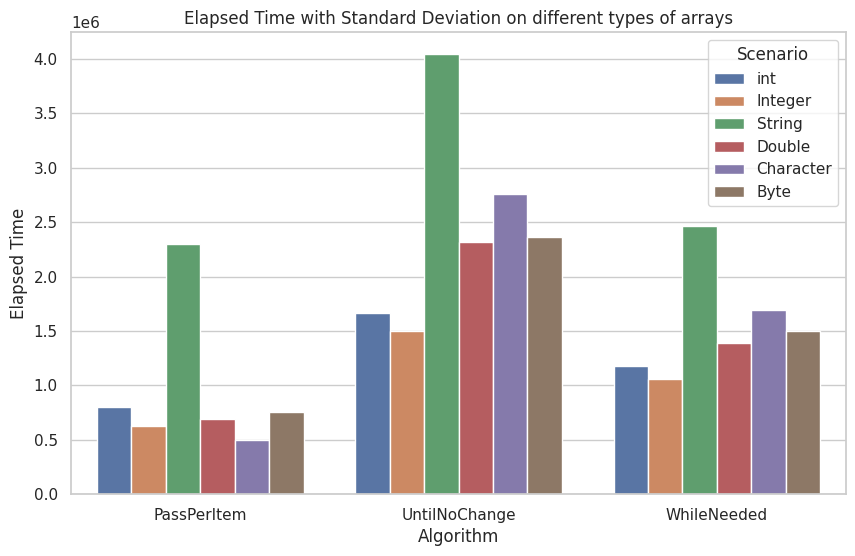
\includegraphics[width=\textwidth]{./data/std_type_array_1000.png}
        \caption{Array dimension = 1000}
    \end{subfigure}
    \hfill
    \begin{subfigure}[b]{0.48\textwidth}
        \centering
        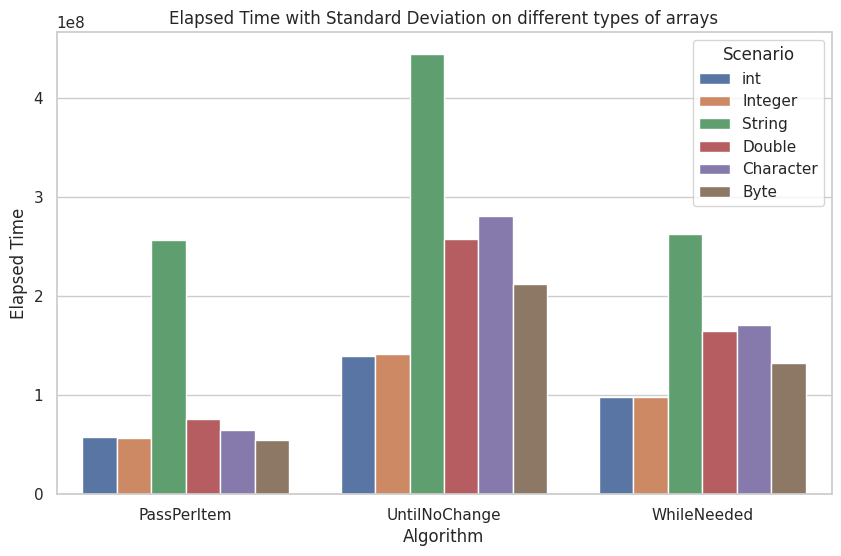
\includegraphics[width=\textwidth]{./data/std_type_array_10000.png}
        \caption{Array dimension = 10000}
    \end{subfigure}
    \caption{STD Mean of elapsed time of Array Type between algorithms}
\end{figure}


\subsection{Descriptive Statistics}
For each group or condition, summarize the set of measured values with a "five-number summary": minimum, first quartile, median, third quartile, and maximum. 

Make sure you explain – in your words – what these statistics mean “in plain English”, but don’t yet interpret them (this is for the Discussion section).

\section{Discussion}
\subsection{Compare Hypothesis to Results}
Provide a brief restatement of the main results from the previous section, and if (or if not) these support your research hypothesis.

If there is a discrepancy between your hypothesis and the results of your experiment, speculate about why you were unable to find evidence to support your hypothesis. 


\subsection{Limitations and Threats to Validity}
Acknowledge any faults or limitations your study has, and how seriously these affect your
results. How could these be remedied in future work?

\subsection{Conclusions}
End with the main conclusions that can be drawn from your study.

\section{Appendix}
\subsection{Materials}
Any documents you used for your informed consent (information sheets, consent) or as part of your apparatus (e.g., manual, hand-out), please include them here.

\subsection{Reproduction Package}
Before, during, and after the experiment you collected all kinds of data. Don't ever throw such data away! Any plots, tables, summaries, and statistics provided in this report should be recreatable from the raw data you have.

If you only collected a small amount of data, put it in this Appendix right here.

If you collected data in forms that are better kept in separate files, then zip up those files, and submit them as a "reproduction package" supporting this report.


\begin{table}[h]
\centering
\resizebox{\textwidth}{!}{%
\begin{tabular}{|c|c|c|c|c|c|c|c|}
\hline
\textbf{ALGORITHM} & \textbf{ELEMENT TYPE ARRAY} & \textbf{ARRAY ORDER} & \textbf{min} & \textbf{Q1} & \textbf{Median} & \textbf{Q3} & \textbf{max} \\
\hline
 & Byte & ... & 3646238.0 & 3756575.0 & 3808821.0 & 3867342.0 & 8357071.0 \\
 & Byte & ... & 2935979.0 & 3019169.0 & 3087391.0 & 3157950.0 & 5288457.0 \\
 & ... & ... & ... & ... & ... & ... \\

 & Character & ... & 3740947.0 & 3846082.0 & 3887237.0 & 3954177.0 & 5698293.0 \\
 & Character & ... & 2893077.0 & 3569756.0 & 3615591.0 & 3720252.0 & 6190770.0 \\
 & ... & ... & ... & ... & ... & ... \\

\textbf{PassPerItem} & Double & ... & 3891059.0 & 4564416.0 & 4708132.0 & 4800219.0 & 7886275.0 \\
 & Double & ... & 4291813.0 & 4516993.0 & 4562359.0 & 4681925.0 & 7910216.0 \\
 & ... & ... & ... & ... & ... & ... \\

 & Integer & ... & 3463755.0 & 3540117.0 & 3598020.0 & 3676245.0 & 4797625.0 \\
 & Integer & ... & 2577646.0 & 2748983.0 & 2819274.0 & 2884196.0 & 4147536.0 \\
 & ... & ... & ... & ... & ... & ... \\

 & String & ... & 6633237.0 & 8086784.0 & 8239239.0 & 8544916.0 & 12653117.0 \\
 & String & ... & 2949728.0 & 3155401.0 & 3213564.0 & 3304831.0 & 5930131.0 \\
 & ... & ... & ... & ... & ... & ... \\

 & int & ... & 3343333.0 & 3482982.0 & 3533921.0 & 3596568.0 & 5805610.0 \\
 & int & ... & 2580467.0 & 2763506.0 & 2829700.0 & 2927601.0 & 4829911.0 \\
 & ... & ... & ... & ... & ... & ... \\
\hline
 & Byte & ... & 5215359.0 & 5426623.0 & 5498350.0 & 5635537.0 & 8687405.0 \\
 & Byte & ... & 5001.0 & 5370.0 & 5719.0 & 8353.0 & 25859.0 \\
 & ... & ... & ... & ... & ... & ... \\

 & Character & ... & 5380184.0 & 5718432.0 & 5805834.0 & 5888586.0 & 9927778.0 \\
 & Character & ... & 4984.0 & 6207.0 & 6542.0 & 9635.0 & 25899.0 \\
 & ... & ... & ... & ... & ... & ... \\

\textbf{UntilNoChange} & Double & ... & 4202655.0 & 5189774.0 & 5401865.0 & 5525006.0 & 7689250.0 \\
 & Double & ... & 4859.0 & 5410.0 & 5645.0 & 5977.0 & 36000.0 \\
 & ... & ... & ... & ... & ... & ... \\

 & Integer & ... & 2500193.0 & 2680410.0 & 2740821.0 & 2833826.0 & 4790417.0 \\
 & Integer & ... & 1921.0 & 2155.0 & 2502.0 & 3209.0 & 23405.0 \\
 & ... & ... & ... & ... & ... & ... \\

 & String & ... & 6416213.0 & 8015924.0 & 8253134.0 & 8469550.0 & 12367124.0 \\
 & String & ... & 3268.0 & 3645.0 & 4342.0 & 5790.0 & 19151.0 \\
 & ... & ... & ... & ... & ... & ... \\

 & int & ... & 2502082.0 & 2618653.0 & 2672308.0 & 2755727.0 & 3633136.0 \\
 & int & ... & 1944.0 & 2200.0 & 2471.0 & 2816.0 & 5192.0 \\
 & ... & ... & ... & ... & ... & ... \\
\hline
 & Byte & ... & 3554805.0 & 3647981.0 & 3705361.0 & 3808088.0 & 5570046.0 \\
 & Byte & ... & 4857.0 & 4981.0 & 7658.0 & 8267.0 & 24460.0 \\
 & ... & ... & ... & ... & ... & ... \\

 & Character & ... & 3479177.0 & 3569511.0 & 3620033.0 & 3686501.0 & 5165470.0 \\
 & Character & ... & 5038.0 & 5285.0 & 5738.0 & 6624.0 & 22933.0 \\
 & ... & ... & ... & ... & ... & ... \\
\hline
\end{tabular}%
}
\caption{Your table caption here}
\label{tab:mytable}
\end{table}


\end{document}
